\chapter{Introduzione alla Return Oriented Programming}
\label{chap:ROP}

\section{Concetti fondamentali per l'applicazione}
\label{sec:fondamentals}

Nel seguente elaborato verrà affrontata la \textbf{Return Oriented Programming}, anche detta ``Programmazione orientata al ritorno''. Essa è una tecnica
mediante la quale un utente malintenzionato potrebbe alterare arbitrariamente il normale flusso di un programma 
senza dover necessariamente iniettare codice di alcun tipo.\cite*{ROP-General}\\
Per comprendere al meglio questa potente tecnica, è necessario primariamente approfondire tutti i concetti su cui essa è fondata, 
analizzando in primo luogo la gestione dell'esecuzione di un qualsiasi programma a livello
di memoria e di registri.\\
L'approccio che verrà impiegato per effettuare gli attacchi si baserà specialmente sulla tipologia di architettura del processore con cui il
software sotto attacco è stato precedentemente sviluppato. Questo perché le istruzioni facenti parte di esso saranno di fondamentale importanza nello sviluppo degli exploit,
come sarà possibile notare nelle successive sezioni.

\subsection{L'architettura del processore}
\label{subsec:arch}
Negli anni, l'attacco basato sulla tecnica ROP si è dimostrato essere applicabile ad un vasto range di architetture differenti \cite*{ROP-architecture}, quali: \textbf{x86}\cite*{ROP-x86},
\textbf{SPARC}\cite*{ROP-General}, \textbf{AtmelAVR}\cite*{ROP-AtmelAVR}, \textbf{Z80}\cite*{ROP-Z80}.\\
Nel seguente lavoro ci si concentrerà sullo studio di questa tecnica applicandola all'architettura \textbf{x86-64}, anche detta ``\textbf{AMD64}'' e ``\textbf{Intel 64}'', ossia l'evoluzione 
della classica \textbf{x86}. Con il passare degli anni essa ha acquisito una grande popolarità, rendendola ad oggi una delle maggiormente supportate e diffuse nei sistemi informatici.\\
Tutto quello che verrà affrontato farà quindi riferimento a questa architettura.

\subsection{La sezione di memoria stack}
\label{subsec:stack}
Il layout di memoria associato ad un qualsiasi programma in linguaggio C eseguito consiste di cinque segmenti \cite{Memory-layout}, chiamati rispettivamente:
\begin{itemize}
    \item \textbf{Stack};
    \item \textbf{Heap};
    \item \textbf{BSS} (Uninitilized data segment);
    \item \textbf{DS} (Initialized data segment);
    \item \textbf{Text}.
\end{itemize} 
In questa porzione di elaborato si cercherà di illustrare la parte di memoria direttamente coinvolta negli attacchi ROP, ossia quella che viene generalmente
chiamata \textbf{stack} o \textbf{execution stack} \cite*{Stack-general}. Questa sezione ha la particolarità di mantenere al suo interno tutte le variabili locali ed i parametri
passati ad una funzione.

\begin{figure}[htbp]
    \centerline{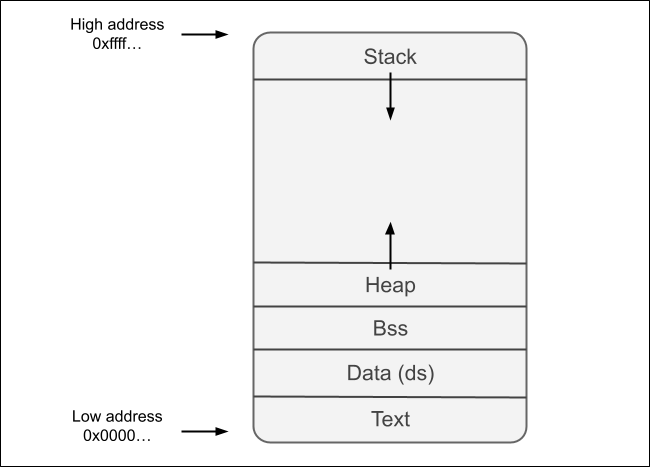
\includegraphics[scale=.5]{images/memory-layout.png}}
    \caption{Rappresentazione del layout di memoria associato ad un programma.}
    \label{fig:memory-layout}
\end{figure}

In questa tipologia di attacchi, la suddetta parte di memoria assume notevole importanza, essa infatti è ciò che consente all'attaccante
di assumere il controllo del flusso del programma. Il suo scopo principale è quello di mantenere traccia 
di ciò che viene comunemente definito ``\textbf{return address}'' o indirizzo di ritorno. Infatti, quando una funzione qualsiasi A viene chiamata %
da una funzione B, la funzione A deve necessariamente passare l'indirizzo su cui ritornare una volta che essa avrà terminato la propria esecuzione, %
e questa importantissima informazione viene memorizzata nello stack. Grazie a ciò sarà possibile recuperare l'indirizzo da cui si era interrotta la 
normale esecuzione del programma per effettuare la subroutine della funzione invocata, direttamente dallo stack, senza alterarne il flusso.\cite*{Stack-general}
Come si vedrà successivamente questo sarà il fulcro su cui verteranno gli attacchi basati sulla \textbf{Return-Oriented Programming}, i quali sfrutteranno alcune 
vulnerabilità conosciute per modificarne il contenuto.\\
Tuttavia, come specificato precedentemente, questa parte di memoria deve mantenere tutte le variabili locali ed eventuali parametri passati ad una
subroutine. Conseguentemente, qualsiasi buffer con relativo contenuto ed eventuali parametri introdotti in fase di chiamata della funzione saranno immagazzinati
al suo interno, rendendola di fatto una zona di memoria tanto importante quanto rischiosa se violata.\\
Una volta compreso com'è strutturato lo stack è necessario approfondire maggiormente il suo funzionamento. Esso, come la struttura
dati omonima, mantiene una politica di gestione degli elementi di tipo \textbf{LIFO} (\textbf{Last In First Out)} e prevede solamente due tipologie di 
operazioni: \textbf{push} e \textbf{pop} \cite*{Stack-operation}.\\
Solitamente queste due operazioni permettono di memorizzare o importare dati da esso collaborando direttamente con i registri del processore, 
i quali saranno approfonditi successivamente. Grazie alla push sarà possibile aggiungere nello stack il valore contenuto all'interno del registro
specificato dall'operazione, mentre la pop consentirà la rimozione dell'ultimo elemento inserito in esso, per caricarlo poi nel registro specificato 
dall'operazione \cite*{Stack-op2}.\\
Quindi, è di fondamentale importanza capire come i registri del processore vengano utilizzati interagendo con lo stack, per comprendere interamente il suo funzionamento.

\subsection{I registri del processore}
\label{subsec:registers}
Un registro del processore è una delle più piccole porzioni di memoria dove poter memorizzare dati facente parte della CPU del computer.
Esso può contenere un'istruzione, un indirizzo di archiviazione o qualsiasi altro tipo di dato (come caratteri o una sequenza di bit) \cite{Register-definition}.\\
È importante che un registro sia abbastanza grande da poter contenere un'istruzione, ad esempio, in un computer a 64 bit come per l'architettura x86-64 un registro deve 
essere lungo almeno 64 bit.\\
Nell'architettura x86-64 i registri vengono solitamente suddivisi in cinque classi principali:
\begin{itemize}
    \item \textbf{General purpose}: \textbf{rax}, \textbf{rbx}, \textbf{rcx}, \textbf{rdx},  \textbf{r8}, \dots, \textbf{r15};
    \item \textbf{Stack}: \textbf{rsp}, \textbf{rbp};
    \item \textbf{Instruction pointer}: \textbf{rip};
    \item \textbf{Indexes}: \textbf{rsi}, \textbf{rdi};
    \item \textbf{Single Instruction Multiple Data}: \textbf{xmm0}, \dots, \textbf{xmm15};
    \item \textbf{Flag register}: \textbf{rFlag}, es: \textbf{ZF}, \textbf{CF}, \textbf{SF}.
\end{itemize}
Inoltre, è possibile accedere specificatamente a delle porzioni dei registri, come si può notare dalla figura \ref{fig:register-partition}.
\begin{figure}[ht]
    \centerline{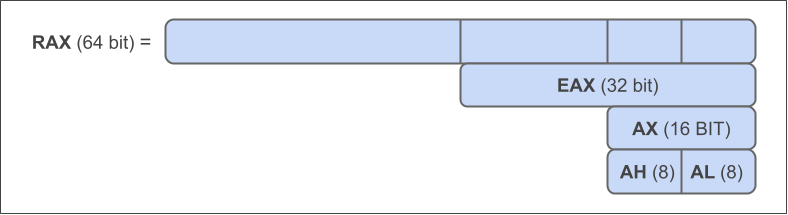
\includegraphics[scale=.6]{images/register-partition.png}}
    \caption{Partizioni accessibili di un registro.}
    \label{fig:register-partition}
\end{figure}
\\Per comprendere il funzionamento della \textbf{ROP}, verrà analizzato principalmente il funzionamento di tre registri: \textbf{rsp} (\textbf{stack pointer}), \textbf{rbp} (\textbf{base pointer}) e \textbf{rip}
(\textbf{instruction pointer}).
I primi due risultano essenziali nella gestione dello stack, ogni qualvolta all'interno di un programma viene richiamata una funzione, un nuovo \textbf{stack frame} specifico sarà creato ed 
essi delimiteranno questa nuova porzione di memoria.
In particolare, il primo registro conterrà l'indirizzo dell'elemento in cima allo stack frame attuale, mentre il secondo conterrà il suo indirizzo di base \cite*{stack-frame-layoutx86-64}.\\
Il \textbf{rip}, invece, conterrà sempre l'indirizzo di memoria su cui risiede la prossima istruzione da eseguire per mantenere il corretto
flusso del programma, cioè il flusso che il creatore del codice si aspetta che sia eseguito.

\section{Funzionamento della tecnica}
\label{sec:func}
Dopo aver introdotto i fondamenti su cui si basa la tecnica di attacco informatico \textbf{Return-Oriented Programming} (\textbf{ROP}), in questa sezione si cercherà di illustrare il 
funzionamento di essa, quindi verranno messi assieme tutti i concetti visti nelle precedenti parti.\\
Un programma ordinario è costituito da una serie di istruzioni assembly, ed ognuna di esse è rappresentata da una serie di byte che, una volta interpretate dal processore, indurranno qualche cambiamento
nello stato del programma. Come accennato precedentemente, il registro \textbf{rip} punterà sempre alla successiva istruzione che dovrà essere eseguita dal processore, una volta terminata quella 
attuale. Questo registro verrà sempre aggiornato dalla CPU dopo ogni istruzione eseguita, in modo che le istruzioni vengano sempre interpretate in sequenza e 
mantenendo il flusso designato \cite*{ROP-General}.
Quando una funzione sarà invocata durante l'esecuzione del codice, com'è stato specificato in precedenza, verrà allocato un nuovo stack frame, e l'indirizzo di ritorno sarà memorizzato 
all'interno di esso \cite*{buffer-overflow}. A questo punto arriviamo alla motivazione per cui la \textbf{Return-Oriented Programming} venga così definita, essa prende il nome dalla celebre istruzione assembly ``\textbf{RETN}'' o
``\textbf{Return from Procedure}'' (``\textbf{ret}'' in x86-64).\\
Al termine di una qualsiasi funzione o subroutine sarà sempre presente questo tipo di istruzione che, una volta raggiunta dal processore, gli imporrà di eseguire una serie di operazioni, quali: il decremento
del registro \textbf{rsp} e soprattutto l'aggiornamento del contenuto del registro \textbf{rip} (che come chiarito in precedenza punterà sempre alla prossima istruzione che la CPU dovrà eseguire) memorizzando in esso
l'indirizzo di ritorno presente in quel momento all'interno dello stack frame attuale.\\
Questa tecnica di exploit sfrutterà tale sequenza di operazioni, l'attaccante dovrà cercare di utilizzare a proprio vantaggio alcune vulnerabilità presenti all'interno del software per sovrascrivere con del codice 
arbitrario l'indirizzo di ritorno memorizzato nello stack, ottenendo così il controllo del flusso di esecuzione del programma.\\
Il reale punto di forza della \textbf{ROP} è la non necessità di iniettare alcun tipo di codice nuovo, utilizzando invece piccole sequenze di istruzioni assembly già disponibili all'interno del binary file del programma
oppure delle librerie collegate all'applicazione, comunemente chiamate \textbf{Gadgets} \cite*{ROP-Basics}.

\subsection{I gadgets}
\label{subsec:gadgets}
Nella precedente sezione sono stati introdotti i \textbf{gadgets}, piccole sequenze di istruzioni assembly che presentano una rilevante particolarità, ossia quella di terminare sempre con un'istruzione \textbf{ret}. 
Esiste anche un'altra tecnica chiamata \label{jop}\textbf{Jump-Oriented Programming} (\textbf{JOP}), che come suggerito dal nome sfrutta sequenze terminanti con un'istruzione \textbf{jmp} \cite*{JOP}\cite*{JOP2}. Essa è una strategia molto efficace, tuttavia 
non verrà trattata in questo elaborato.\\
I \textbf{gadgets} sono uno strumento molto versatile per l'attaccante, il quale potrà utilizzarli una volta preso il controllo dello stack per effettuare qualsiasi operazione esso voglia riutilizzando il codice già presente.\\

\begin{figure}[ht]
    \centerline{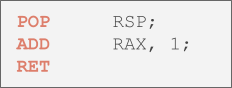
\includegraphics[scale=.6]{images/Gadget.png}}
    \caption{Esempio di un ipotetico Gadget nell'architettura x86-64.}
    \label{fig:Gadget}
\end{figure}

Esistono due tipologie di \textbf{gadgets} o sequenze: le ``\textbf{Unintented Istruction Sequences}'' e le ``\textbf{Intented Istruction Sequences}'' \cite*{ROP-architecture}.\\
poiché nell'architettura x86-64 i \textbf{gadgets} non si limitano ad essere solamente sequenze di istruzioni esistenti. Essendo quest'ultime di dimensioni variabili potrebbe esistere una potenziale sequenza utile inattesa, prendendone
semplicemente una intenzionale partendo da un offset differente da quello aspettato \cite*{Gadgets-unintended}. 

\begin{figure}[ht]
    \centerline{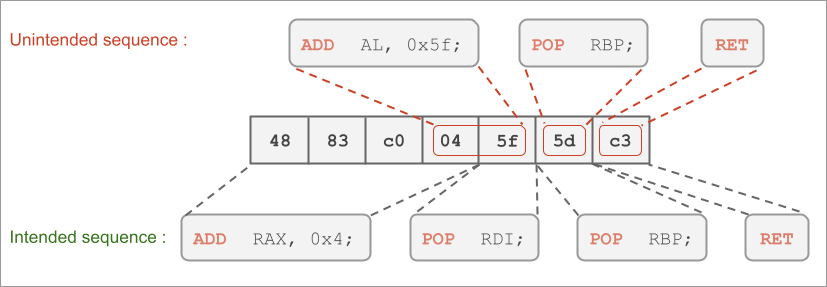
\includegraphics[scale=.6]{images/Unintended-seq.png}}
    \caption{Esempio di un gadget ricavato da una sequenza intenzionale, prendendo un offset differente da quello previsto.}
    \label{fig:Unintended-seq}
\end{figure}

È anche questa una delle motivazioni che ha suggerito dopo decenni di ricerche, come la \textbf{ROP} sia Turing Completa \cite*{ROP-x86}\cite*{ROP-General}, quindi in linea 
teorica è possibile assemblare qualsiasi tipo di programma arbitrario utilizzando solamente questi \textbf{gadgets} \cite*{ROP-General2}. Essendo infatti queste sequenze tutte composte da una serie di istruzioni sempre
terminanti da una \textbf{ret} (o \textbf{jmp}), l'attaccante potrà concatenare assieme questi gadget inserendoli opportunamente all'interno dello stack, formando quella che viene comunemente definita \textbf{ROP-Chain} \cite*{ROP-Chain}.

\begin{figure}[h]
    \centerline{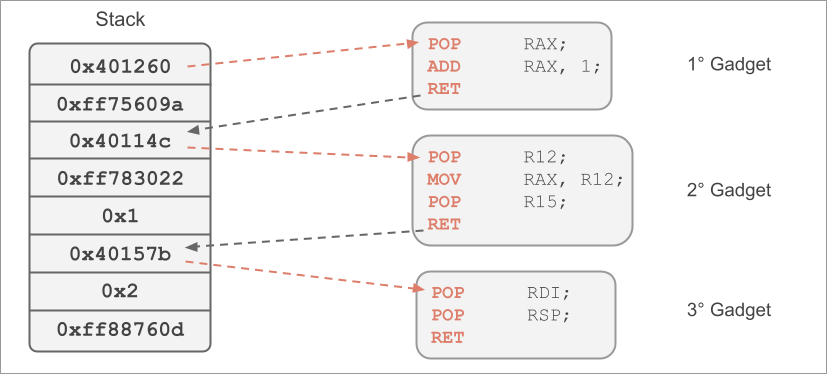
\includegraphics[scale=.6]{images/Rop-Chain.png}}
    \caption{Esempio di una possibile \textbf{ROP chain} caricata nello stack.}
    \label{fig:ROP-chain}
\end{figure}

Ora non resta che capire come un attaccante possa reperire queste essenziali sequenze di istruzioni. A tale scopo, sono stati ideati molti strumenti in grado di identificarli all'interno dei binary file.
Alcuni dei più conosciuti ed utilizzati sono: \textbf{\textit{ROPgadget}} di Jonathan Salwan \cite*{ROPgadget}, \textbf{\textit{Ropper}} di Sascha Schirra \cite*{Ropper} e \textbf{\textit{Radare2}} del gruppo Radare \cite*{Radare2}.\\
Questi strumenti verranno approfonditi successivamente visto che saranno principalmente utilizzati per effettuare i diversi test.
Ora che è stato chiarito il funzionamento di questa potente tecnica d'attacco è necessario comprendere in quali situazioni essa possa essere applicata, ossia di fronte a quali vulnerabilità risulti 
particolarmente efficace.


